\documentclass{standalone}
\usepackage{tikz}
\usetikzlibrary{patterns, positioning}


\begin{document}
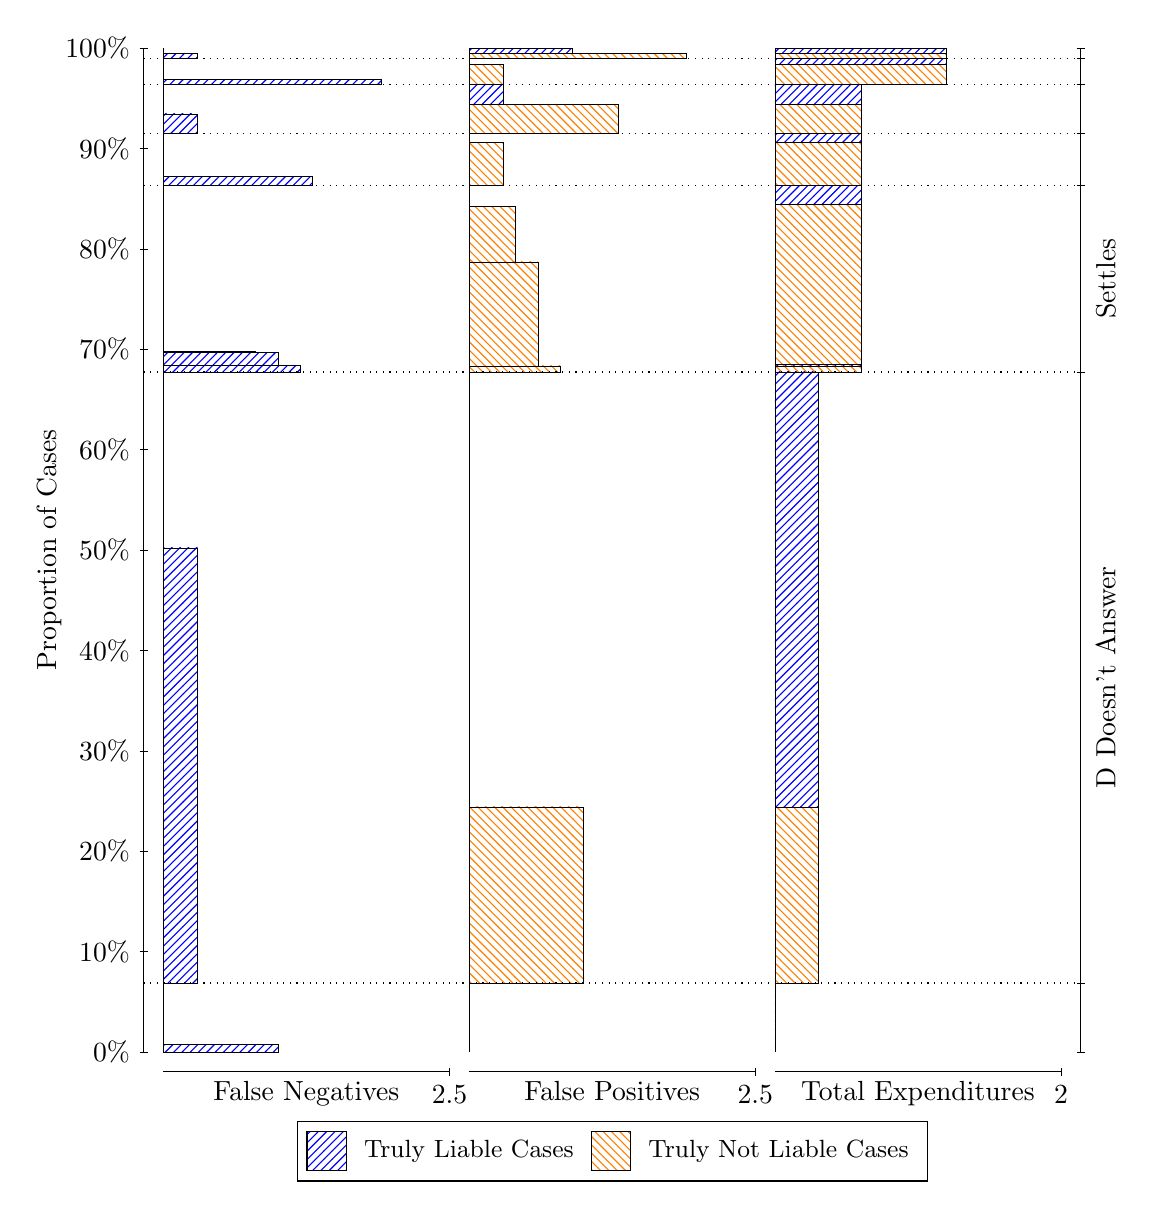
\begin{tikzpicture}
\draw[black, very thin] (1.5,1.75) -- (1.5,14.5);
\node[rotate=90, text=black, anchor=center] at (0.3, 8.125) {Proportion of Cases};
\draw[black, very thin] (1.45,1.75) -- (1.55,1.75);
\node[text=black, anchor=east] at (1.45, 1.75) {0\%};
\draw[black, very thin] (1.45,3.025) -- (1.55,3.025);
\node[text=black, anchor=east] at (1.45, 3.025) {10\%};
\draw[black, very thin] (1.45,4.3) -- (1.55,4.3);
\node[text=black, anchor=east] at (1.45, 4.3) {20\%};
\draw[black, very thin] (1.45,5.575) -- (1.55,5.575);
\node[text=black, anchor=east] at (1.45, 5.575) {30\%};
\draw[black, very thin] (1.45,6.85) -- (1.55,6.85);
\node[text=black, anchor=east] at (1.45, 6.85) {40\%};
\draw[black, very thin] (1.45,8.125) -- (1.55,8.125);
\node[text=black, anchor=east] at (1.45, 8.125) {50\%};
\draw[black, very thin] (1.45,9.4) -- (1.55,9.4);
\node[text=black, anchor=east] at (1.45, 9.4) {60\%};
\draw[black, very thin] (1.45,10.675) -- (1.55,10.675);
\node[text=black, anchor=east] at (1.45, 10.675) {70\%};
\draw[black, very thin] (1.45,11.95) -- (1.55,11.95);
\node[text=black, anchor=east] at (1.45, 11.95) {80\%};
\draw[black, very thin] (1.45,13.225) -- (1.55,13.225);
\node[text=black, anchor=east] at (1.45, 13.225) {90\%};
\draw[black, very thin] (1.45,14.5) -- (1.55,14.5);
\node[text=black, anchor=east] at (1.45, 14.5) {100\%};

\draw[black, very thin] (13.4,1.75) -- (13.4,14.5);
\draw[black, very thin] (13.35,1.75) -- (13.45,1.75);
\node[anchor=west] at (13.35, 1.75) {};
\draw[black, very thin] (13.35,2.6263) -- (13.45,2.6263);
\node[anchor=west] at (13.35, 2.6263) {};
\draw[black, very thin] (13.35,10.386) -- (13.45,10.386);
\node[anchor=west] at (13.35, 10.386) {};
\draw[black, very thin] (13.35,12.753) -- (13.45,12.753);
\node[anchor=west] at (13.35, 12.753) {};
\draw[black, very thin] (13.35,13.418) -- (13.45,13.418);
\node[anchor=west] at (13.35, 13.418) {};
\draw[black, very thin] (13.35,14.034) -- (13.45,14.034);
\node[anchor=west] at (13.35, 14.034) {};
\draw[black, very thin] (13.35,14.364) -- (13.45,14.364);
\node[anchor=west] at (13.35, 14.364) {};
\draw[black, very thin] (13.35,14.5) -- (13.45,14.5);
\node[anchor=west] at (13.35, 14.5) {};

\draw[black, very thin, pattern color=blue, pattern=north east lines] (1.75,1.75) rectangle (3.2033,1.8422);
\draw[black, very thin, pattern color=orange, pattern=north west lines] (1.75,1.8422) rectangle (1.75,2.6263);
\draw[black, very thin, pattern color=blue, pattern=north east lines] (1.75,2.6263) rectangle (2.186,8.1508);
\draw[black, very thin, pattern color=orange, pattern=north west lines] (1.75,8.1508) rectangle (1.75,10.386);
\draw[black, very thin, pattern color=blue, pattern=north east lines] (1.75,10.386) rectangle (3.494,10.469);
\draw[black, very thin, pattern color=blue, pattern=north east lines] (1.75,10.469) rectangle (3.2033,10.63);
\draw[black, very thin, pattern color=blue, pattern=north east lines] (1.75,10.63) rectangle (2.9127,10.65);
\draw[black, very thin, pattern color=orange, pattern=north west lines] (1.75,10.65) rectangle (1.75,12.753);
\draw[black, very thin, pattern color=blue, pattern=north east lines] (1.75,12.753) rectangle (3.6393,12.867);
\draw[black, very thin, pattern color=orange, pattern=north west lines] (1.75,12.867) rectangle (1.75,13.418);
\draw[black, very thin, pattern color=blue, pattern=north east lines] (1.75,13.418) rectangle (2.186,13.663);
\draw[black, very thin, pattern color=orange, pattern=north west lines] (1.75,13.663) rectangle (1.75,14.034);
\draw[black, very thin, pattern color=blue, pattern=north east lines] (1.75,14.034) rectangle (4.5113,14.1);
\draw[black, very thin, pattern color=orange, pattern=north west lines] (1.75,14.1) rectangle (1.75,14.364);
\draw[black, very thin, pattern color=blue, pattern=north east lines] (1.75,14.364) rectangle (2.186,14.434);
\draw[black, very thin, pattern color=orange, pattern=north west lines] (1.75,14.434) rectangle (1.75,14.5);
\draw[black, very thin, pattern color=orange, pattern=north west lines] (5.6333,1.75) rectangle (5.6333,2.5341);
\draw[black, very thin, pattern color=blue, pattern=north east lines] (5.6333,2.5341) rectangle (5.6333,2.6263);
\draw[black, very thin, pattern color=orange, pattern=north west lines] (5.6333,2.6263) rectangle (7.0867,4.862);
\draw[black, very thin, pattern color=blue, pattern=north east lines] (5.6333,4.862) rectangle (5.6333,10.386);
\draw[black, very thin, pattern color=orange, pattern=north west lines] (5.6333,10.386) rectangle (6.796,10.463);
\draw[black, very thin, pattern color=orange, pattern=north west lines] (5.6333,10.463) rectangle (6.5053,11.783);
\draw[black, very thin, pattern color=orange, pattern=north west lines] (5.6333,11.783) rectangle (6.2147,12.49);
\draw[black, very thin, pattern color=blue, pattern=north east lines] (5.6333,12.49) rectangle (5.6333,12.753);
\draw[black, very thin, pattern color=orange, pattern=north west lines] (5.6333,12.753) rectangle (6.0693,13.304);
\draw[black, very thin, pattern color=blue, pattern=north east lines] (5.6333,13.304) rectangle (5.6333,13.418);
\draw[black, very thin, pattern color=orange, pattern=north west lines] (5.6333,13.418) rectangle (7.5227,13.789);
\draw[black, very thin, pattern color=blue, pattern=north east lines] (5.6333,13.789) rectangle (6.0693,14.034);
\draw[black, very thin, pattern color=orange, pattern=north west lines] (5.6333,14.034) rectangle (6.0693,14.297);
\draw[black, very thin, pattern color=blue, pattern=north east lines] (5.6333,14.297) rectangle (5.6333,14.364);
\draw[black, very thin, pattern color=orange, pattern=north west lines] (5.6333,14.364) rectangle (8.3947,14.43);
\draw[black, very thin, pattern color=blue, pattern=north east lines] (5.6333,14.43) rectangle (6.9413,14.5);
\draw[black, very thin, pattern color=orange, pattern=north west lines] (9.5167,1.75) rectangle (9.5167,2.5341);
\draw[black, very thin, pattern color=blue, pattern=north east lines] (9.5167,2.5341) rectangle (9.5167,2.6263);
\draw[black, very thin, pattern color=orange, pattern=north west lines] (9.5167,2.6263) rectangle (10.062,4.862);
\draw[black, very thin, pattern color=blue, pattern=north east lines] (9.5167,4.862) rectangle (10.062,10.386);
\draw[black, very thin, pattern color=orange, pattern=north west lines] (9.5167,10.386) rectangle (10.607,10.463);
\draw[black, very thin, pattern color=blue, pattern=north east lines] (9.5167,10.463) rectangle (10.607,10.482);
\draw[black, very thin, pattern color=orange, pattern=north west lines] (9.5167,10.482) rectangle (10.607,12.51);
\draw[black, very thin, pattern color=blue, pattern=north east lines] (9.5167,12.51) rectangle (10.607,12.753);
\draw[black, very thin, pattern color=orange, pattern=north west lines] (9.5167,12.753) rectangle (10.607,13.304);
\draw[black, very thin, pattern color=blue, pattern=north east lines] (9.5167,13.304) rectangle (10.607,13.418);
\draw[black, very thin, pattern color=orange, pattern=north west lines] (9.5167,13.418) rectangle (10.607,13.789);
\draw[black, very thin, pattern color=blue, pattern=north east lines] (9.5167,13.789) rectangle (10.607,14.034);
\draw[black, very thin, pattern color=orange, pattern=north west lines] (9.5167,14.034) rectangle (11.697,14.297);
\draw[black, very thin, pattern color=blue, pattern=north east lines] (9.5167,14.297) rectangle (11.697,14.364);
\draw[black, very thin, pattern color=orange, pattern=north west lines] (9.5167,14.364) rectangle (11.697,14.43);
\draw[black, very thin, pattern color=blue, pattern=north east lines] (9.5167,14.43) rectangle (11.697,14.5);
\draw[black, dotted] (1.5,2.6263) -- (13.4,2.6263);
\draw[black, dotted] (1.5,10.386) -- (13.4,10.386);
\draw[black, dotted] (1.5,12.753) -- (13.4,12.753);
\draw[black, dotted] (1.5,13.418) -- (13.4,13.418);
\draw[black, dotted] (1.5,14.034) -- (13.4,14.034);
\draw[black, dotted] (1.5,14.364) -- (13.4,14.364);
\draw[black, very thin] (1.75,1.5) -- (5.3833,1.5);
\node[text=black, anchor=north] at (3.5667, 1.5) {False Negatives};
\draw[black, very thin] (5.3833,1.45) -- (5.3833,1.55);
\node[text=black, anchor=north] at (5.3833, 1.45) {2.5};

\draw[black, very thin] (5.6333,1.5) -- (9.2667,1.5);
\node[text=black, anchor=north] at (7.45, 1.5) {False Positives};
\draw[black, very thin] (9.2667,1.45) -- (9.2667,1.55);
\node[text=black, anchor=north] at (9.2667, 1.45) {2.5};

\draw[black, very thin] (9.5167,1.5) -- (13.15,1.5);
\node[text=black, anchor=north] at (11.333, 1.5) {Total Expenditures};
\draw[black, very thin] (13.15,1.45) -- (13.15,1.55);
\node[text=black, anchor=north] at (13.15, 1.45) {2};


\node[text=black, centered, rotate=90] at (13.72, 6.5064) {D Doesn't Answer};
\node[text=black, centered, rotate=90] at (13.72, 11.57) {Settles};





\draw (7.449999999999999,1.5) node[draw=none] (baseCoordinate) {};
\begin{scope}[align=center]
        \matrix[scale=0.5, draw=black, below=0.5cm of baseCoordinate, nodes={draw}, column sep=0.1cm]{
            \node[rectangle, draw, minimum width=0.5cm, minimum height=0.5cm, pattern color=blue, pattern=north east lines] {}; &
            \node[draw=none, font=\small, text=black] (B) {Truly Liable Cases}; &
            \node[rectangle, draw, minimum width=0.5cm, minimum height=0.5cm, pattern color=orange, pattern=north west lines] {}; &
            \node[draw=none, font=\small, text=black] (B) {Truly Not Liable Cases}; \\
            };
\end{scope}

\end{tikzpicture}
\end{document}